\documentclass[reprint, english,notitlepage]{revtex4-1}  % defines the basic parameters of the document
% if you want a single-column, remove reprint

% allows special characters (including æøå)
\usepackage[utf8]{inputenc}
\usepackage [norsk]{babel} %if you write norwegian
%\usepackage[english]{babel}  %if you write english


%% note that you may need to download some of these packages manually, it depends on your setup.
%% I recommend downloading TeXMaker, because it includes a large library of the most common packages.

\usepackage{physics,amssymb}  % mathematical symbols (physics imports amsmath)
\usepackage{graphicx}         % include graphics such as plots
\usepackage{xcolor}           % set colors
\usepackage{hyperref}         % automagic cross-referencing (this is GODLIKE)
\usepackage{tikz}             % draw figures manually
\usepackage{listings}         % display code
\usepackage{subfigure}        % imports a lot of cool and useful figure commands
\usepackage{verbatim}
\usepackage{adjustbox}

% defines the color of hyperref objects
% Blending two colors:  blue!80!black  =  80% blue and 20% black
\hypersetup{ % this is just my personal choice, feel free to change things
    colorlinks,
    linkcolor={red!50!black},
    citecolor={blue!50!black},
    urlcolor={blue!80!black}}

%% Defines the style of the programming listing
%% This is actually my personal template, go ahead and change stuff if you want
\lstset{ %
	inputpath=,
	backgroundcolor=\color{white!88!black},
	basicstyle={\ttfamily\scriptsize},
	commentstyle=\color{magenta},
	language=Python,
	morekeywords={True,False},
	tabsize=4,
	stringstyle=\color{green!55!black},
	frame=single,
	keywordstyle=\color{blue},
	showstringspaces=false,
	columns=fullflexible,
	keepspaces=true}

\begin{document}



\title{Elektromagnetisk stråling}
\date{\today}
\author{Knadidatnr.: 15889}
\affiliation{Institute of Theoretical Astrophysics, University of Oslo}
\email{textme@astro.uio.no}


\newpage

\begin{abstract}
Jeg har studert lys som er observert fra en fjern stjerne på ti forskjellige dager over en toukers periode. Ved å se på Doppler-forskyvning av en spektrallinje har jeg klart å beregne stjernens hastighet i forhold til oss ved hver av de ti målingene. På bakgrunn av dette kunne jeg slå fast at stjernen beveger seg bort fra oss med en gjennomsnittshastighet på ca. 15km/s. Den beveger seg i tillegg i bane med svært kort omløpsperiode, bare rundt 10 dager, og høy banefart, ca. 1.5km/s. Dette indikerer tilstedeværelsen av et annet massivt legeme like i nærheten.

For å finne eksakte verdier for bølgelengden til absorpsjonslinjen i det Doppler-forskjøvede spekteret brukte jeg minste kvadraters metode. Termiske bevegelser i gassene på stjernens overflate, og annen støy, gjør at dette kan være vanskelig å gjøre med øyemål. Jeg har anvendt modeller for fluks og støy som bygger på normalfordelingen, noe som har vist seg å være fornuftige antakelser.
\end{abstract}
\maketitle                                % creates the title, author, date & abstract



\section{Introduksjon}
\label{sect:intro}

I dette prosjektet skal jeg studere lys som er observert fra en fjern stjerne. Jeg har måledata fra 10 dager, og skal ved å studere spektrallinjer for mottatt fluks prøve å finne stjernens hastighet i forhold til oss på jorda ved forskjellige tidspunkter. Dette kan videre brukes til å påvise planeter i bane rundt stjernen, og finne massen og innholdet i atmosfæren til eventuelle planeter (se \citep{part1C} og \citep{paper1C}).

Alt vi kan måle fra fjerne solsystemer og galakser er egenskaper ved den elektromagnetiske strålingen vi mottar fra dem. Å utvikle teorien og teknologien som brukes til å studere denne strålingen er er en avgjørende del av innsatsen som må legges ned for å øke vår forståelse av den delen av universet som ligger utenfor vår egen atmosfære. Dette prosjektet utforsker hva som er mulig å lære om stjerner og planeter som ligger langt unna vårt eget solsystem, og beskriver, sammen med arbeidene som refereres til, helhetlig de mest anvendte metodene for slike analyser.




\section{Teori}

Ved å observere lyset som når oss fra fjerne stjerner kan vi finne ut hvilken fart stjernen har i
 forhold til oss her på jorda. På grunn av Doppler-Effekten vil lys sendt ut fra en kilde som
 beveger seg bort fra oss bli rødforskjøvet og lys fra en kilde som beveger seg mot oss vil bli
 blåforskjøvet. Likning \ref{eq:doppler} forteller oss hvordan vi kan finne hastigheten til
 lyskilden relativt til oss:

\begin{equation}
  \label{eq:doppler}
  \frac{\lambda - \lambda_0}{\lambda_0} = \frac{v_r}{c}
\end{equation}
Her er $\lambda$ bølgelengden til en absorpsjonslinje for det observerte lyset og $\lambda_0$ er
 bølgelengden vi måler for den samme absorpsjonslinjen i laboratoriet på jorda. $v_r$ er farten
 til stjerna i forhold til oss og $c$ er lysfarten. Negativt fortegn på $v_r$ betyr at lyskilden er på vei mot oss, positivt fortegn betyr at den er på vei bort fra oss.

Den øverste illustrasjonen i figur \ref{fig:theoretical_flux} viser hvordan fluksen vi mottar fra
 en stjerne kan se ut. Modellen vi antar for fluksen er gitt i likning \ref{eq:flux_model}, se
 \citep{part1D}.

\begin{equation}
  \label{eq:flux_model}
  F^{\text{model}}(\lambda) = F_{\text{max}} + (F_{\text{min}} - F_{\text{max}}) e^{-(\lambda - \lambda_{\text{center}})^2/(2 \sigma^2)}
\end{equation}
Her er $F_{\text{max}}$ kontinuumsfluksen (som er 1 for relativ fluks), $F_{\text{min}}$ er den minste verdien
 for den observerte fluksen, $\lambda$ er bølgelengde, $\lambda_{\text{center}}$ er bølgelengden som
 svarer til $F_{\text{min}}$ og $\sigma$ er et mål på bredden av dalen rundt $\lambda_{\text{center}}$. I
 ekte målinger for fluks har vi støy som jeg antar er normalfordelt med middelverdi 0 og konstant standardavvik.

Stjerna sender ut lys fordi den har høy temperatur som et resultat av fusjonsprosesser. Denne termiske energien frigis som stråling. Grunnen til at vi ser absorpsjonslinjer er at lyset fra stjerna passerer gjennom gasser, mest sannsynlig rundt stjerna, på vei til oss. Molekylene i gassen absorberer fotoner med visse bølgelengder slik at det er mindre lys med akkurat disse bølgelengdene som når oss. Gassmolekylene som sender ut lyset fra stjernas overflate beveger seg med forskjellige hastigheter. Bølgelengden til lyset som blir sendt ut vil være ulikt for molekyler som beveger seg med forskjellige hastigheter, på grunn av Doppler-forskyvningen.

Vi antar at hastighetene til molekylene i gassen er normalfordelt. Det betyr at de fleste partiklene har hastighet i forhold til massesenteret til stjernen like rundt 0 i radiell retning sett fra observatøren. Absorpsjonslinjen til lyset fra disse partiklene er forskjøvet til $\lambda_{\text{center}}$. I tillegg har vi mange partikler som beveger seg med hastighet ulik 0 i radiell retning i forhold til massesenteret til stjernen. Lyset fra alle disse partiklene vil være forskjøvet til andre verdier enn $\lambda_{\text{center}}$. Det gjør at figuren har en slik bred dal rundt $\lambda_{\text{center}}$ fordi det ikke bare er lys med bølgelengde $\lambda_{\text{center}}$ som blir absorbert, men også lys med litt mindre og litt større bølgelengde. Flukskurven, som er beskrevet ved likning \ref{eq:flux_model}, viser en normalfordeling ettersom det er en direkte konsekvens av molekylenes hastighet i radiell retning, som vi antar er normalfordelt$^{\citep{part1A}}$.

 \begin{figure}
   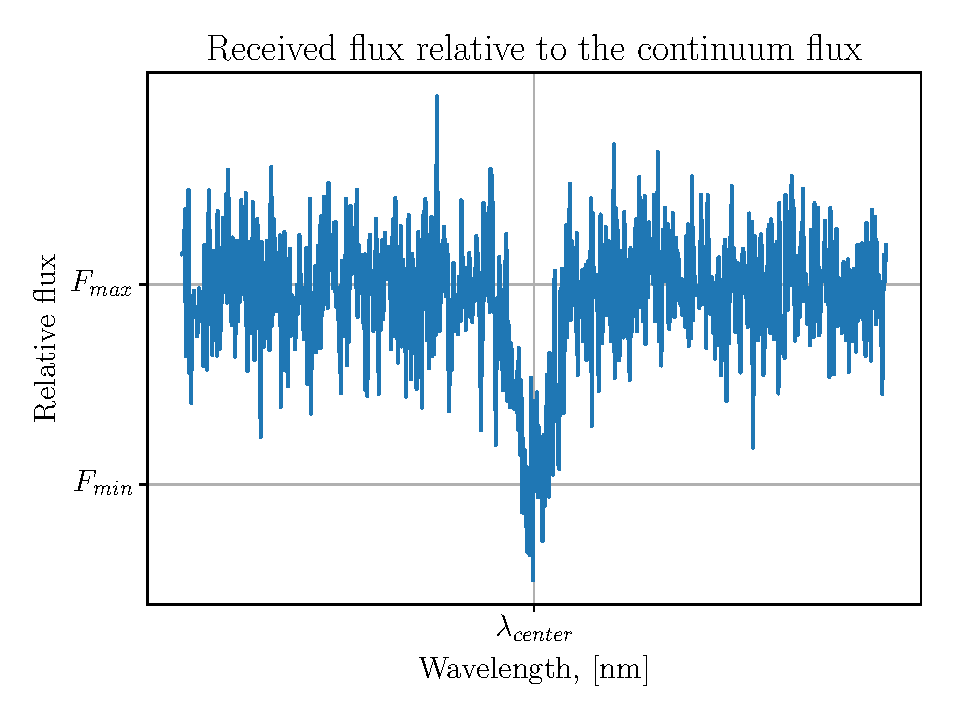
\includegraphics[width=\linewidth]{../output/plots/theoretical_flux_noise.pdf}
   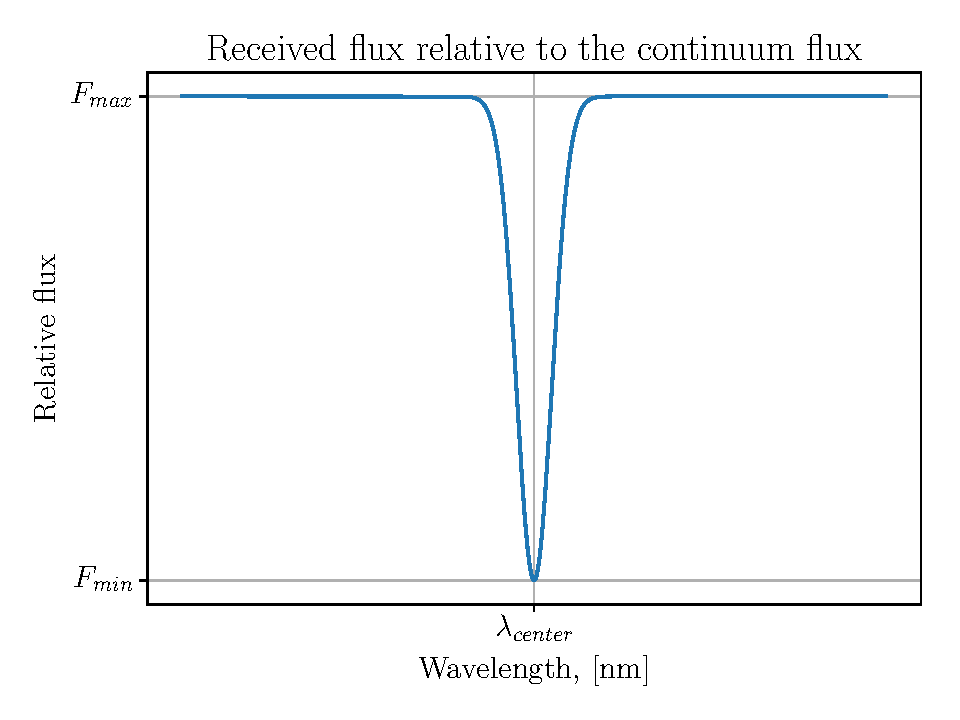
\includegraphics[width=\linewidth]{../output/plots/theoretical_flux_nonoise.pdf}
   \caption{Fluksen vi mottar fra en stjerne som funksjon av bølgelengde. Nederst har vi verdiene uten støy. Øverst er det med normalfordelt støy, slik dataen vi mottar ser ut.}
   \label{fig:theoretical_flux}
 \end{figure}




\section{Metode}

Jeg har måledata som viser den
 relative fluksen til lyset fra en stjerne over et intervall av bølgelengden for 10 forskjellige dager. Dataen jeg har fått er illustrert i figur \ref{fig:spectra}. Dersom vi har en absorpsjonslinje
 ved en bestemt bølgelengde og vi kjenner bølgelengden for den samme absorpsjonslinjen når vi måler
 den i laboratoriet på jorda kan vi finne stjernas hastighet relativt til oss ved å løse likning
 \ref{eq:doppler} for $v_r$:

\begin{equation}
  \label{eq:v_r}
  v_r = \frac{\lambda - \lambda_0}{\lambda_0} c
\end{equation}

Ved å se på dataen for fluksen kan vi bestemme med øyemål verdier for $\lambda_{\text{center}}$ fra
 likning \ref{eq:flux_model}, se figur \ref{fig:theoretical_flux}. Mer nøyaktige verdier kan
 finnes ved å prøve å bestemme de verdiene for $F_{\text{min}}$, $\sigma$ og $\lambda_{\text{center}}$ som gjør
 at uttrykket for $F^{\text{model}}$ best beskriver de måledataene vi har observert. Det jeg ønsker å
 gjøre er å prøve modellen med mange forskjellige kombinasjoner av ulike verdier for disse
 parametrene og finne den beste kombinasjonen. For å finne fram til disse verdiene velger jeg en
 øvre og nedre grense for hver av parametrene slik at jeg er sikker på at den virkelige verdien
 jeg er ute etter ligger innenfor intervallet. Deretter tester jeg modellen med 30 jevnt fordelte
 verdier innenfor dette intervallet, og plukker ut det settet med verdier som gir best tilnærming.


For å finne øvre og nedre grense for intervallene til parametrene bruker jeg en automatisk
 algoritme. Siden det er relativ fluks vi måler er $F_{\text{max}} = 1$ for alle stjernene. Jeg antar at
 støyen er normalfordelt med middelverdi 0 og samme standardavvik hele tiden, slik at jeg kan
 anta at den minste verdien til $F^{obs}$ ligger i nærheten av den reelle minsteverdien
 $F_{\text{min}}$. Jeg legger derfor intervallet for $\lambda_{\text{center}}$ slik at bølgelengden for den
 minste verdien av $F^{obs}$ ligger i midten. For å finne den reelle minsteverdien til
 fluksen tar jeg først gjennomsnittet av de 3 minste verdiene vi har målt for å redusere effekten
 av et par målinger med veldig stor støy, dersom det skulle være noen i dette området. Jeg leter
 deretter etter den reelle minsteverdien i området mellom 60\% og 100\% av avstanden mellom
 $F_{\text{max}}$ og den middelverdien jeg nå fikk. Når det gjelder $\sigma$, så kan vi utnytte at
 modellen er bygget på normalfordeling. Det betyr at 99.7\% skal være innenfor $3 \sigma$. Jeg
 kan derfor trygt sette største mulige verdi for $\sigma$ til for eksempel 0.01 fordi vi ser på den observerte dataen at
 kurven har flatet ut i god tid før man har beveget seg et avstand 0.03 fra $\lambda_{\text{center}}$.
 (Et høyere tak enn 0.01 er brukt for å produsere resultatene i artikkelen, men ved å sette taket
 til 0.01 kunne resultatene blitt mer presise). Hastighetene til gassmolekylene i stjerna avhenger av temperaturen til stjerna, hvilket betyr at $\sigma$ også er temperaturavhengig. Temperaturen endrer seg ikke fra dag til dag, og jeg kan dermed anta at sigma ikke endrer seg nevneverdig fra dag til dag heller. Jeg bruker derfor det samme intervallet for $\sigma$ hver dag.

Jeg ønsker å finne de verdier for $F_{\text{min}}$, $\sigma$ og $\lambda_{\text{center}}$ som gjør at $F^{\text{model}}$ best beskriver den observerte dataen. For å finne ut hvilken kombinasjon som gir minst avvik fra måledataen bruker jeg minste
 kvadraters metode. Som et mål på feilen til modellen med gitte parametre bruker jeg
 kvadratavviket $(F^{obs} (\lambda) - F^{\text{model}} (\lambda, F_{\text{min}}, \sigma, \lambda_{\text{center}}))^2$,
 som gir et tall på hvor langt unna modellen er den målte verdien for én bestemt bølgelengde.
 Målet er å mimimere den totale feilen som er gitt ved summen av alle kvadratavvikene over alle
 bølgelengder:
 \begin{equation}
   \label{eq:error}
   \Delta (F_{\text{min}}, \sigma, \lambda_{\text{center}}) = \sum_{\lambda} (F^{obs} - F^{\text{model}})^2
 \end{equation}




\section{Resultat}

Resultatene fra minste
 kvadraters metode for dataen fra hver av dagene finnes i tabell \ref{fig:table}. Begge er i
 Appendix. Figur \ref{fig:modelled_flux} viser hvordan den modellerte løsningen passer med
 måledataen for dag 0.

Det er i utgangspunktet verdiene for $\lambda_{\text{center}}$ vi er interessert i for å kunne lære om
 bevegelsen til stjernen og eventuelle planeter i nærheten. Ved å anvende likning \ref{eq:v_r} på
 disse verdiene for $\lambda_{\text{center}}$ får jeg den radielle hastighetene til stjernen i forhold
 til oss ved hver av målingene. (Vi vet at $\lambda_0 = 656.3$nm). Resultatene er gitt i tabell
 \ref{fig:table_vels}, og er illustrert i figur \ref{fig:radial_vels}. Av figuren ser det ut til
 at stjernen beveger seg bort fra oss med en pekuliærhastighet på ca. 15km/s og har en banefart
 på rundt 1.5km/s. Til sammenlikning er banefarten til vår sol ca. 20km/s i forhold til
 gjennomsnittshastigheten til andre stjerner i nabolaget$^{\citep{wiki}}$

\begin{table}
\begin{adjustbox}{width=\linewidth}
\begin{tabular}{||c | c | c||}
\hline
Day & $v_r$ by-eye, [km/s] & $v_r$ least squares, [km/s] \\ \hline\hline
0 & 14.2 & 13.8    \\ \hline
2 & 15.5 & 15.6    \\ \hline
3 & 16.9 & 16.4    \\ \hline
5 & 15.5 & 16.0    \\ \hline
6 & 14.2 & 14.2    \\ \hline
8 & 12.8 & 13.3    \\ \hline
9 & 13.7 & 13.7    \\ \hline
11 & 15.1 & 15.6    \\ \hline
13 & 16.9 & 16.5    \\ \hline
14 & 16.0 & 15.7    \\ \hline
\end{tabular}
\end{adjustbox}
\caption{Resultatene av å anvende likning \ref{eq:v_r} på dataene for mottatt fluks. Andre kolonne er ved øyemål for $\lambda_{\text{center}}$, tredje kolonne er ved minste kvadraters metode for å finne $\lambda_{\text{center}}$ (se tabell \ref{fig:table}).}
\label{fig:table_vels}
\end{table}

\begin{figure}
  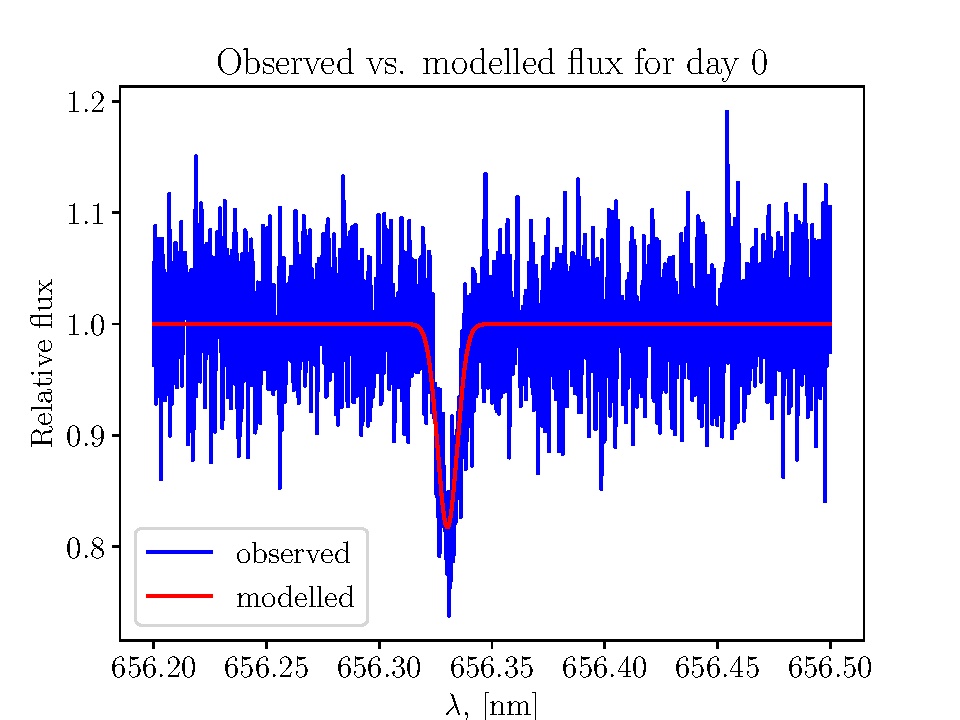
\includegraphics[width=\linewidth]{../output/plots/modelled_flux.pdf}
  \caption{Observerte og modellerte verdier for fluksen observert på dag 0.}
  \label{fig:modelled_flux}
\end{figure}

\begin{figure}
  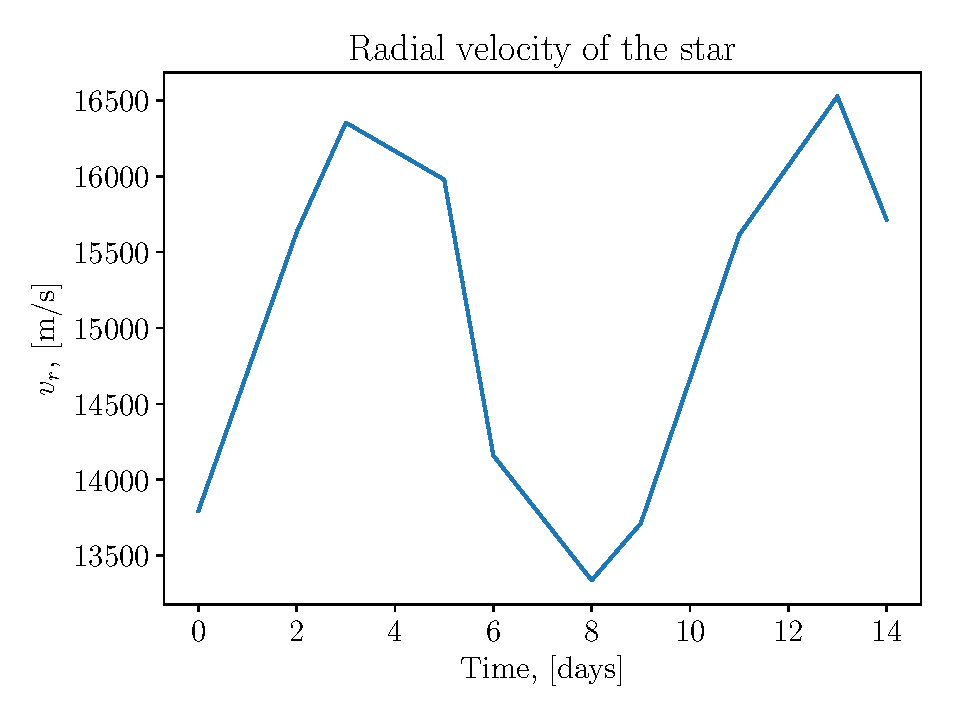
\includegraphics[width=\linewidth]{../output/plots/radial_vels.pdf}
  \caption{Den radielle hastigheten til stjernen, funnet ved hjelp av minste kvadraters metode.}
  \label{fig:radial_vels}
\end{figure}


\section{Diskusjon}

Når jeg analyserte fluksdataen med minste kvadraters metode bruke jeg 30 testverdier for hver av
 de ukjente parametrene $F_{\text{min}}$, $\sigma$ og $\lambda_{\text{center}}$. Ved å øke til 40 testverdier
 innenfor det samme intervallet forventet jeg å få mer nøyaktige svar. Det viste seg imidlertid
 at dette bare førte til en endring på mellom 0.00003\% og 0.00013\% av $\lambda_{\text{center}}$ som er
 den parameteren vi bryr oss om. Jeg konkluderer derfor med at 30 testverdier gir så godt som så
 presise svar vi kan finne, og jeg er komfortabel med å bruke 30 testverdier videre. Som nevnt i
 metode-delen oppdaget jeg etter implementering av algoritmen at den øvre grensen for $\sigma$
 trygt kunne vært satt en del lavere enn den verdien jeg brukte. Dette ville antakeligvis gitt
 noe mer nøyaktige resultater.

Ved å se på figur \ref{fig:radial_vels} ser vi tydelige periodiske svingninger i hastigheten til
 stjernen. Det betyr at stjernen beveger seg i bane og har en komponent av banehastigheten som er
 parallell med vår siktlinje. For at stjernen skal gå i bane, må den påvirkes av en
 gravitasjonskraft som antakelig kommer fra en nærliggende planet. Det virker derfor som at
 stjernen har en planet i bane rundt seg. Illustrasjonen viser en bemerkelsesverdig kort omløpsperiode for stjernen, bare rundt 10 dager, særlig når man tar i betrakning at banefarten til tider er minst 1.5km/s. Det må være et svært massivt legeme nært denne stjernen for å gi denne type bevegelse. Vi kunne brukt datapunktene for hastigheten til å finne den minste mulige massen til dette legemet, se \citep{paper1C}.




\onecolumngrid
\vspace{1cm} % some extra space


\begin{thebibliography}{}
\bibitem[Hansen (2017)]{part1A} Hansen, F. K.,  2017, Forelesningsnotat 1A i kurset AST2000
\bibitem[Hansen (2017)]{part1C} Hansen, F. K.,  2017, Forelesningsnotat 1C i kurset AST2000
\bibitem[Hansen (2017)]{part1D} Hansen, F. K.,  2017, Forelesningsnotat 1D i kurset AST2000
\bibitem[15889 (2019)]{paper1C} 15889,  2019, Ekstrasolare planeter
\bibitem[5]{wiki} Solen, https://no.wikipedia.org/wiki/Solen, Lest 17.10.19

\end{thebibliography}



\section{Appendix}

\begin{figure}
  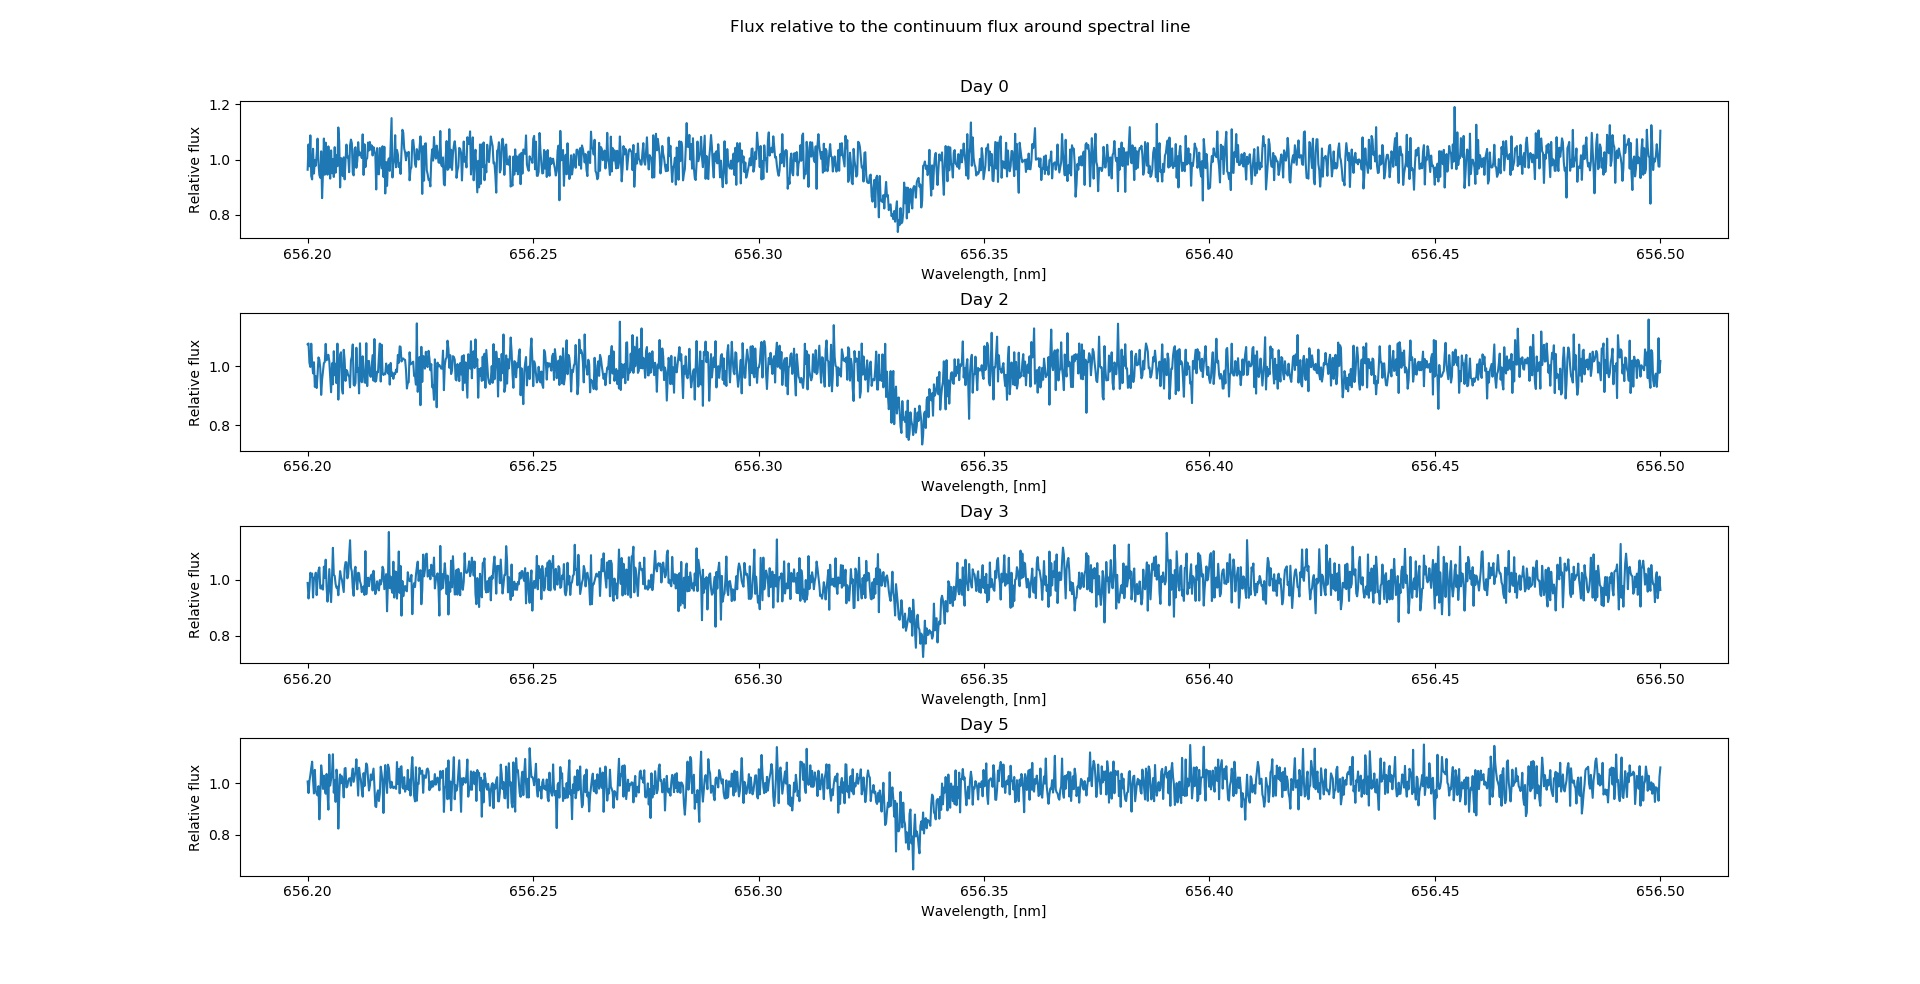
\includegraphics[width=15cm]{../output/plots/Spectra_1.jpg}
  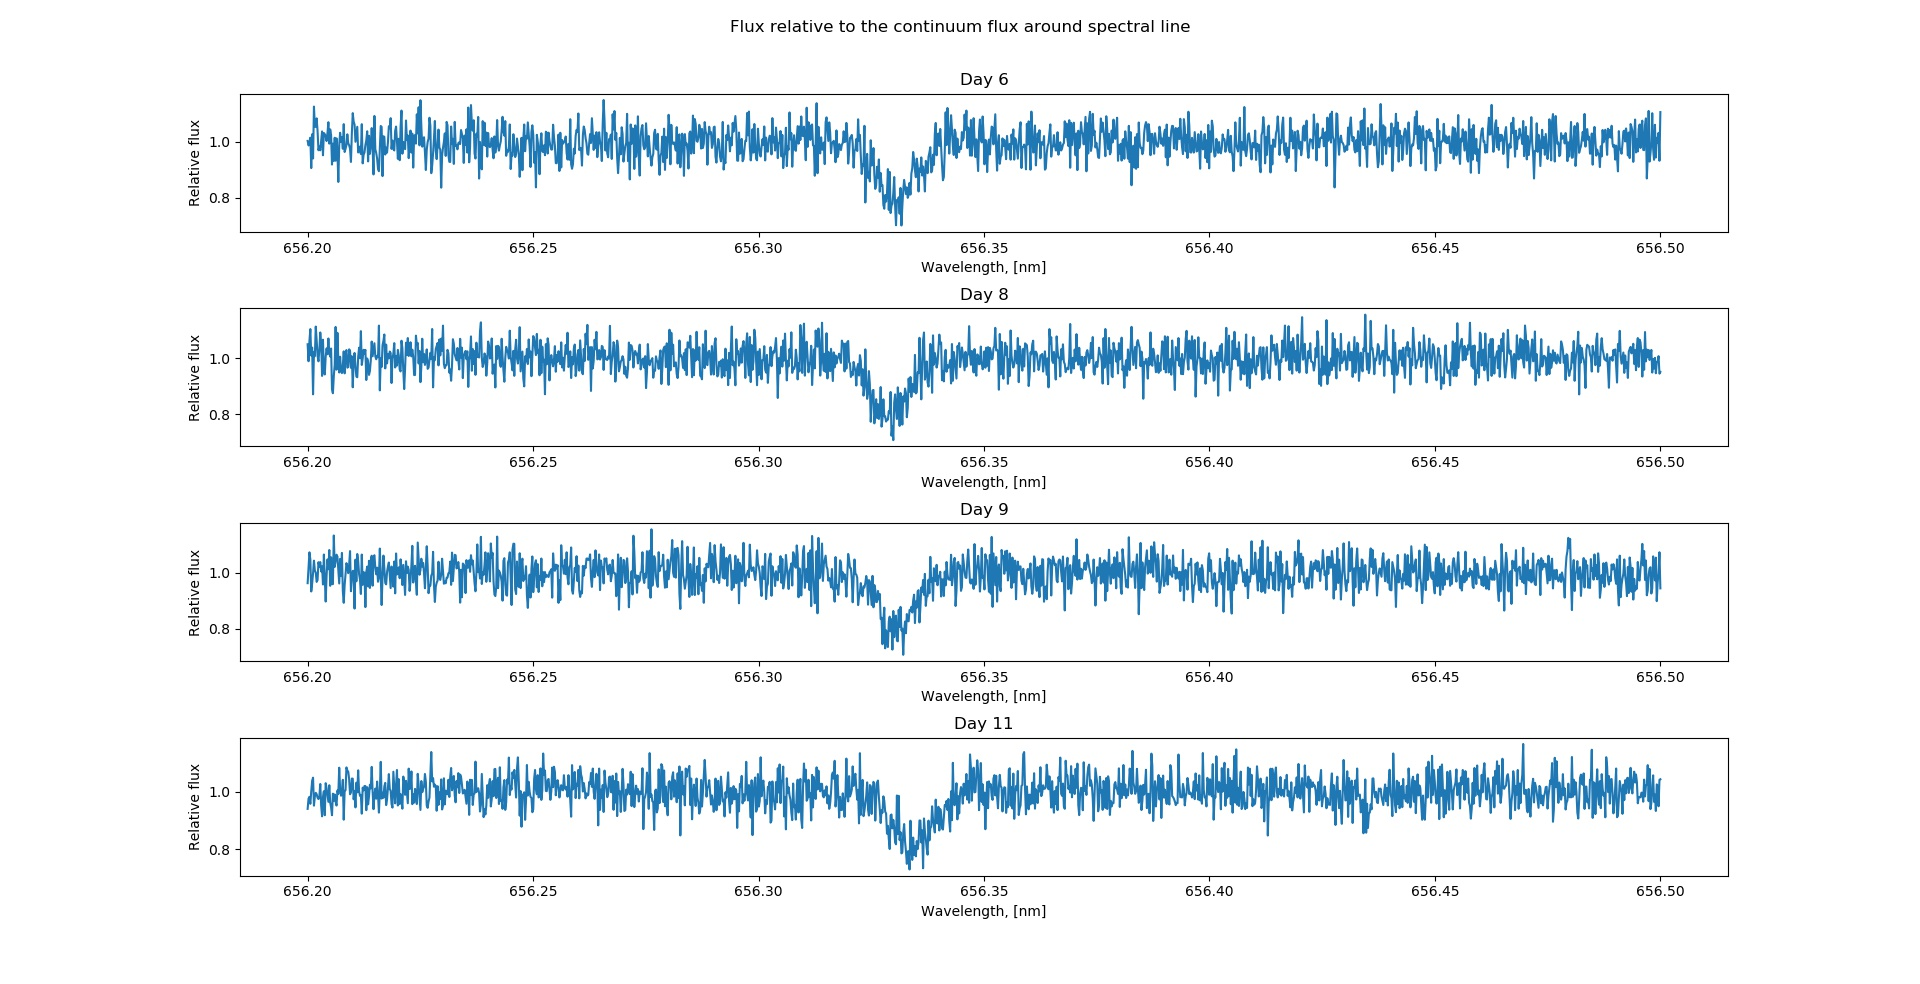
\includegraphics[width=15cm]{../output/plots/Spectra_2.jpg}
  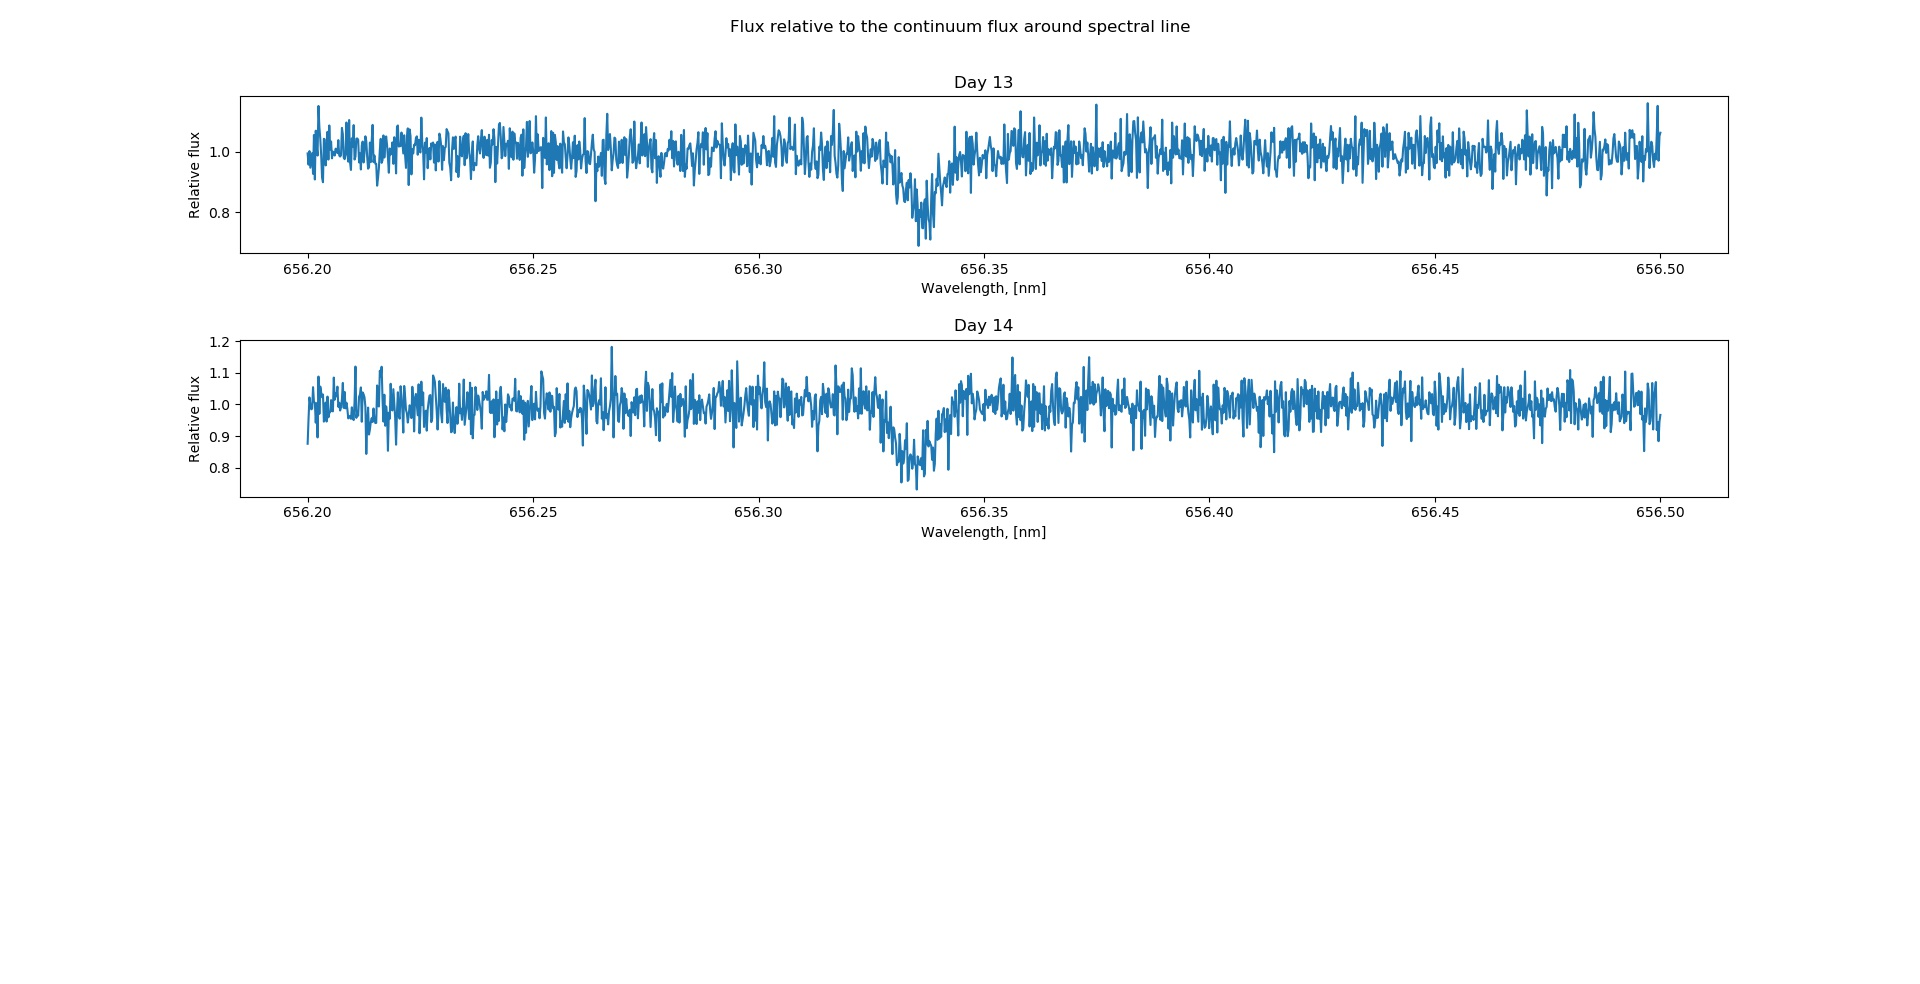
\includegraphics[width=15cm]{../output/plots/Spectra_3.jpg}
  \caption{Den relative fluksen som funksjon av bølgelengde for lyset vi har mottatt fra stjernen de 10 dagene.}
  \label{fig:spectra}
\end{figure}


\begin{table}[p]
\begin{adjustbox}{width=1\textwidth}
\begin{tabular}{||c | c | c | c | c||}
\hline
Day & $F_{\text{min}}$ & $\sigma$ & $\lambda$, [nm] & $\Delta$ \\ \hline\hline
0 & 0.81742 & 0.00438 & 656.33020 & 3.73793    \\ \hline
2 & 0.81084 & 0.00438 & 656.33422 & 3.55735    \\ \hline
3 & 0.81249 & 0.00438 & 656.33580 & 3.75985    \\ \hline
5 & 0.81334 & 0.00438 & 656.33498 & 3.69936    \\ \hline
6 & 0.79401 & 0.00438 & 656.33100 & 4.00017    \\ \hline
8 & 0.80051 & 0.00438 & 656.32920 & 3.65960    \\ \hline
9 & 0.80140 & 0.00438 & 656.33002 & 3.83682    \\ \hline
11 & 0.80581 & 0.00438 & 656.33418 & 3.88872    \\ \hline
13 & 0.80998 & 0.00438 & 656.33618 & 3.65010    \\ \hline
14 & 0.81709 & 0.00438 & 656.33440 & 3.68551    \\ \hline
\end{tabular}
\end{adjustbox}
\caption{Tabell som viser resultatene av minste kvadraters metode anvendt på dataen registrert for hver av de 10 dagene. $F^{\text{model}}$ er testet med alle kombinasjoner av 30 forskjellige verdier for $F_{\text{min}}$, $\sigma$ og $\lambda_{\text{center}}$. Den beste kombinasjonen ga totalt avvik $\Delta$ mellom $F^{obs}$ og $F^{\text{model}}$.}
\label{fig:table}
\end{table}



\end{document}
